\documentclass[a4paper,14pt]{extarticle}
\usepackage{cmap}				% To be able to copy-paste russian text from pdf			
\usepackage[utf8]{inputenc}
\usepackage[T1]{fontenc}
\usepackage[margin=1in]{geometry}
\usepackage[english, russian]{babel}

\usepackage[hyphens]{url}
\urlstyle{same}
\usepackage{hyperref}

\usepackage{multirow}
\usepackage{graphicx}
\usepackage{caption}
\usepackage{amsmath}
\usepackage{mathtools}

\usepackage{tikz}
\usepackage{pgfplots}
\usepgfplotslibrary{groupplots,colorbrewer,dateplot,statistics}

%\def\ishtml{1}
\ifdefined\ishtml
  % HTML mode
  \newcommand{\urlnote}[2]{\href{#2}{#1}} % Make cool link 
  \newcommand{\smallsep}{thinspace} % to be replaced with unicode 8239 later
\else
  % PDF mode
   \usepackage{libertine}
   \usepackage{libertinust1math}
   \newcommand{\urlnote}[2]{#1\endnote{\url{#2}}}  % Put URLs to endnotes
   \newcommand{\smallsep}{\kern 0.1em}
\fi

% Move footnotes to end of document
\usepackage[backref=true]{enotez}
\DeclareTranslation{russian}{enotez-title}{Примечания}

\usepackage[
	output-decimal-marker={,},
	group-separator={\smallsep},
	group-minimum-digits=3
]{siunitx}

% Shoot me if I know a better way to make decimal groups of two
\newcommand{\rateone}[1]{\num{#1}}
\newcommand{\ratetwo}[2]{\num{#1}\smallsep#2}
\newcommand{\ratethree}[3]{\num{#1}\smallsep#2\smallsep#3}

\newcommand{\ru}[1]{\begin{otherlanguage}{russian}#1\end{otherlanguage}}
\newcommand{\en}[1]{\begin{otherlanguage}{english}#1\end{otherlanguage}}
\newcommand{\ruen}[2]{#1 (\en{#2})}

\usepackage[style=alphabetic, backend=biber]{biblatex}
\addbibresource{index.bib}
\renewcommand*{\bibfont}{\small}
\setcounter{biburllcpenalty}{9000}
\setcounter{biburlucpenalty}{9500}

\author{Артём Бакулин}
\date{\today}

\title{Соотношение <<цена-прибыль>> Шиллера и пузыри на рынке акций}

% Try small font in captions
\usepackage[font=small]{caption}

% No extra line skip in itemize
\usepackage{enumitem}
\setlist{nosep}

\begin{document}

\maketitle
\thispagestyle{empty}

\begin{figure}[h]
\centering
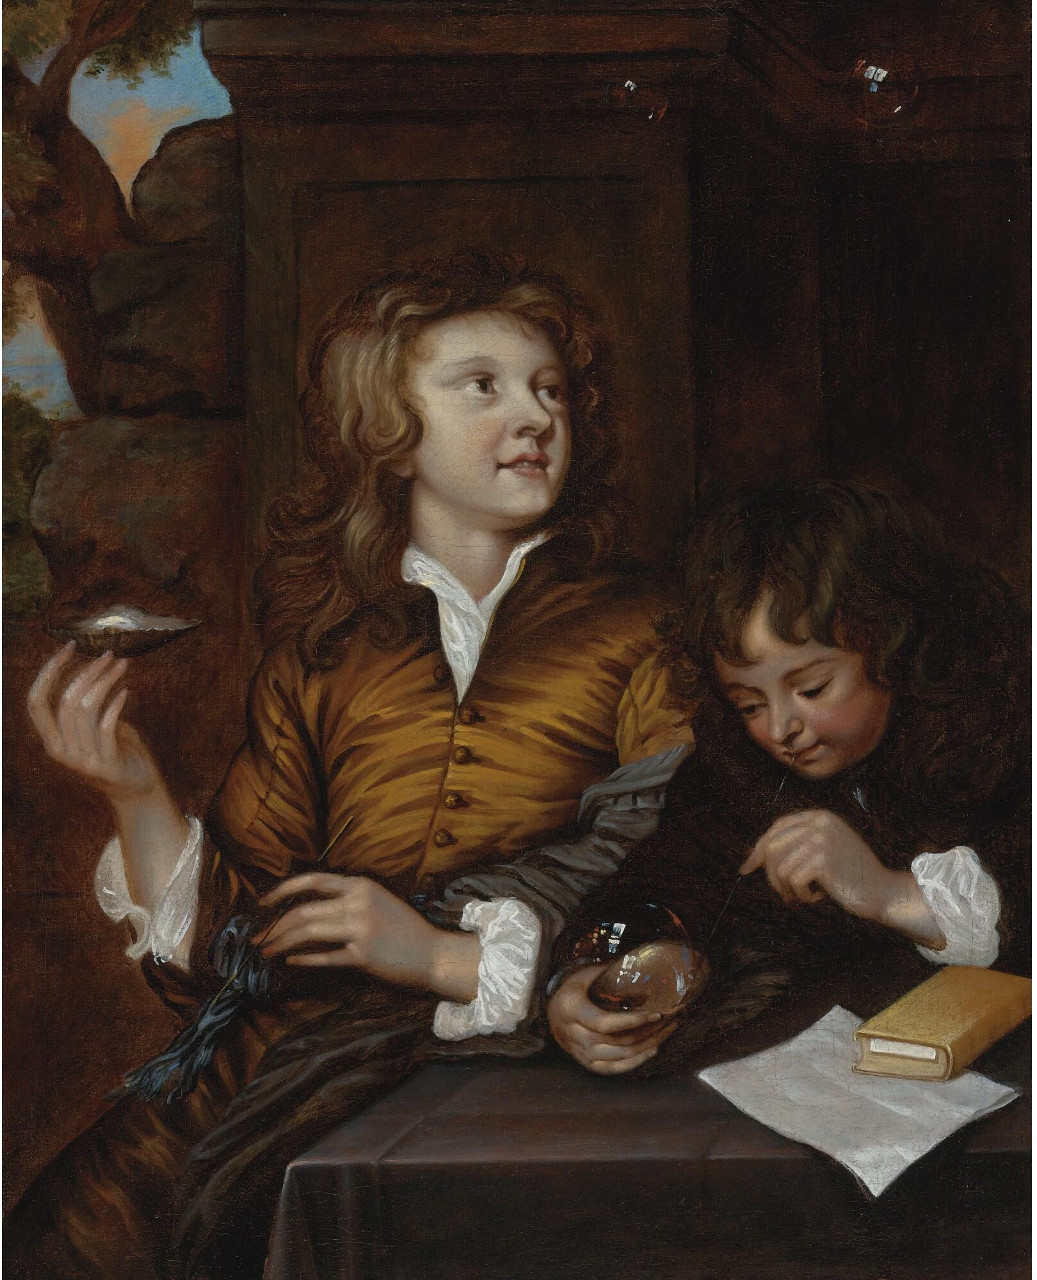
\includegraphics[height=14.9cm]{img/two_boys_blowing_bubbles.jpg}
\captionsetup{labelformat=empty}
\caption{\small{
    Адриан Ханнеман.
    \urlnote{Два мальчика, выдувающие пузыри}
    {https://www.sothebys.com/en/auctions/ecatalogue/2010/old-master-19th-century-european-art-n08611/lot.746.html}.
    ок. 1630 г. Музей искусств Нортона, Уэст-Палм-Бич.
}}
\end{figure}
\setcounter{figure}{0}
\newpage

\section*{Введение}
Пару месяцев назад на Хабре вышла статья
\urlnote{<<На фондовом рынке США сформировался пузырь небывалых размеров>>}
{https://habr.com/ru/post/541114/}. Согласно этой статье, <<мультипликаторы 
находятся на исторических максимумах>>, так что <<большой кризис неизбежен>>.

Один из мультипликаторов, на который ссылается статья --- это известное
соотношение <<цена-прибыль>> Шиллера. Честно говоря, я уже сбился со счёта, 
сколько раз за последние годы я читал апокалиптические прогнозы, основанные на 
индикаторе Шиллера. Чтобы выяснить, насколько можно верить этим прогнозам, я 
решил наконец-то почитать работы Шиллера и других исследователей. Оказалось, 
что недавно даже сам Шиллер написал, что такой прямолинейный взгляд на 
показатель <<цена-прибыль>> может быть весьма спорным. 

В этой статье я расскажу, как устроен многострадальный индикатор Шиллера, 
почему сам Шиллер не вполне поддерживает всёпропальщицкие предсказания, есть ли 
статистическая связь между индикатором и долгосрочной доходностью рынка акций, 
и можно ли на ней заработать. Спойлер: скорее всего, философский камень 
инвестиций всё ещё не найден, а высокое соотношение <<цена-прибыль>> в первую 
очередь связано с низким процентными ставками.

\section*{Соотношение <<цена-прибыль>> и соотношение Шиллера}

Пожалуй, самая заезженная формула в инвестициях --- это соотношение 
\ruen{<<цена/прибыль>>}{Price/Earnings, P/E}. Чтобы посчитать соотношение 
<<цена-прибыль>> рынка акций, нужно разделить капитализацию рынка (суммарную 
стоимость всех акций всех компаний) $P$ на общую прибыль всех компаний $E$. 
Например, если все акции всех компаний из индекса S\&P\,500 вместе взятые стоят 
\dollars{30} триллионов, и компании заработали в прошлом году \dollars{0.75} 
триллиона, то соотношение P/E равно $30/0.75 = 40$. Покупая сейчас индекс 
акций, вы покупаете компании за 40 годовых прибылей.

Чтобы прочувствовать физический смысл соотношения P/E, представьте, что вы 
купили небольшой бизнес, например кафе. Кафе приносит, скажем, \num{500 
000} рублей чистой прибыли в год, а купили вы его за \num{20 000 000} рублей. 
Соотношение P/E, следовательно, равно 40. Пройдет 40 лет, прежде чем прибыль 
от кафе отобьёт начальные вложения. Если вам кажется, что купить кафе за 40 
годовых прибылей --- сомнительная затея, то я с вами согласен. Поэтому я 
отчасти могу понять финансовых аналитиков, которых озадачивает показатель P/E 
рынка акций США. Действительно, всё ли в порядке с головой у инвесторов, 
которые покупают компании за 30, 35, 40 годовых прибылей? Давайте разбираться.

Поскольку простая формула P/E выглядит недостаточно солидно, обычно аналитики 
заменяют прибыль прошлого года $E$ на среднюю прибыль за последние 10 лет. Надо 
признать, что в этом есть смысл. Прибыли компаний меняются с течением времени. 
В какие-то годы экономика на подъёме, и прибыли компаний оказываются выше 
среднего. В не столь удачные годы экономика замедляется, и вместе с ней 
снижаются прибыли компаний. Если взять среднее за достаточно длинный период, 
лет 10--12, то мы сгладим колебания, связанные с экономическими циклами.

Нужно только не забыть, что из-за инфляции один доллар 10 лет назад и один 
доллар в прошлом году --- это немного разные доллары. Чтобы складывать яблоки с 
яблоками, нужно домножить прибыли прошлых лет на накопленную инфляцию. 
Обозначим $E_{1}$ суммарную прибыль всех компаний за прошлый год, $E_2$ --- 
суммарную прибыль за предпоследний год, и так далее до $E_{10}$ --- годовой 
прибыли компаний 10 лет назад. Также обозначим инфляцию за последние 10 лет 
$I_{10}$, за последние 9 лет --- $I_9$ и так далее до $I_1$. Например, если 
$I_5=1.2$, то за пять последних лет цены выросли в 1.2 раза. Тогда мы сможем 
посчитать среднюю прибыль компаний за последние 10 лет  $E'$:
\begin{align*}
E' &= \frac{E_1I_1 + E_2I_2 + ... + E_{10}I_{10}}{10}
\end{align*}

Если эту среднюю прибыль за 10 лет $E'$ подставить в <<обычное>> соотношение 
P/E, то получится соотношение \ruen{<<цена-прибыль>> с поправкой на 
цикличность}{cyclically-adjsuted price/earnings, CAPE}. Его ещё иногда называют 
\ruen{соотношением Шиллера}{Shiller ratio} в честь одного из первооткрывателей, 
профессора \ruen{Роберта Шиллера}{Robert Shiller} \cite{campbell1988dividend}:
\begin{align}
\text{CAPE} = \frac{P}{E'} = \frac{10P}{E_1I_1 + E_2I_2 + ... + E_{10}I_{10}}
\label{cape_formula}
\end{align}

Теперь, когда мы разобрались, что такое соотношение Шиллера, самое время 
посмотреть, каким оно было в прошлом и какое оно сейчас. Пожалуйста, уведите от 
экрана беременных женщин и детей. Сейчас вы увидите шокирующий график, который, 
по мнению некоторых  финансовых аналитиков, предсказывает неминуемый крах 
фондового рынка США. Внимание на рисунок \ref{shiller_pe_historical_chart}.



\newcommand{\dotWithNumber}[5] {
        \node[
            circle,
            fill,
            inner sep = 2pt,
            color = #3
        ]
        at (axis cs: #1, #2) {};
        
        \node[
            anchor=#5
        ]
        at (axis cs: #1, #2)
        {#4};
}



\begin{figure}[ht]
\centering
\begin{tikzpicture}
\begin{axis}[
    width=\textwidth - 0.5cm,
    date coordinates in=x,
    date ZERO=1880-01-01,
    xtick={1880-01-01,1900-01-01,1920-01-01,1940-01-01,1960-01-01,1980-01-01,2000-01-01,2020-01-01},
    minor xtick={1890-01-01,1910-01-01,1930-01-01,1950-01-01,1970-01-01,1990-01-01,2010-01-01},
    xticklabel=\year,
    grid=both,
    xmin=1880-01-01,
    xmax=2026-01-01,
    ylabel={Соотношение P/E с поправкой на цикличность (CAPE)},
]
    
    \newcommand{\capeDotAndNumber}[2]{
         \dotWithNumber{#1}{#2}{Set1-B}{#2}{south}
    }
    
        \addplot[
            color = Set1-B,
            line width = 1pt
        ]
        table[
            x = month,
            y = shiller_cape,
            col sep = comma
        ]
        {data/shiller_cape.csv};        

        \capeDotAndNumber{1929-09-01}{32.6}        
        \capeDotAndNumber{1999-12-01}{44.2}
        \capeDotAndNumber{2021-03-01}{35.0}
\end{axis}
\end{tikzpicture}
\caption{Соотношение <<цена/прибыль>> с поправкой на цикличность (CAPE) для 
рынка акций США. Данные: Robert Shiller \cite{shillerOnline}.}
\label{shiller_pe_historical_chart}
\end{figure}

Текущее значение (35.0 по состоянию на март 2021 года) выглядит довольно 
высоким по историческим меркам. В прошлом лишь дважды акции стоили дороже, чем 
30 годовых прибылей: в 1929-м аккурат перед Великой депрессией и в конце 1990-х 
на пике пузыря интернет-компаний. И вот история повторяется в третий раз. Снова 
на рынке акций надулся пузырь. Мы стоим на пороге финансовой катастрофы, после 
которой живые позавидуют мёртвым. Скажите, вам уже страшно?

Впрочем, я бы не спешил накрываться белой простынёй и медленно ползти на 
кладбище. Ирония в том, что аналитики продолжают ссылаться на авторитет Шиллера 
(нобелевский лауреат, как-никак), хотя он сам не так давно написал, что, 
возможно, никакого пузыря-то и нет. По его словам, высокое соотношение CAPE 
может быть связано с низкими процентными ставками и не обязательно является 
предвестником финансового шторма \cite{shiller2020cape}.

\section*{Цены акций и процентные ставки. Формула Гордона}

Чтобы понять аргументацию Шиллера и соавторов, нам нужно разобраться, как 
связаны цены акций и процентные ставки.

Представим, что некая компания зарабатывает прибыль $E$, которую полностью 
выплачивает в виде дивидендов. Компания развивается, и каждый год прибыль 
растёт на $g$ процентов. Первая выплата $E$ долларов случится через год, через 
два года компания выплатит $E(1+g)$, через три года $E(1+g)^2$ и так далее до 
бесконечности. Компания никогда не разорится и будет ежегодно выплачивать  
растущие дивиденды. Внимание, вопрос: сколько стоит такая компания?

На первый взгляд, компания в будущем выплатит акционерам бесконечное количество 
долларов, поэтому её цена --- тоже бесконечность. Это простое рассуждение 
неверно, потому что оно суммирует будущие доллары, которые вовсе не равны 
сегодняшним.

Во-первых, инфляция со временем съедает покупательную способность денег. Скорее 
всего, через 10 лет вы купите на \dollars{100} меньше товаров, чем могли бы 
купить на \dollars{100} сегодня. Во-вторых, даже если инфляции нет вовсе, то 
всё равно люди при прочих равных предпочитают потребление сегодня потреблению в 
будущем. Поэтому доллары, полученные от нашей компании через 10 лет, менее 
ценны, чем доллары, полученные через 5 лет, и, разумеется, менее ценны, чем 
сегодняшние доллары.

Чтобы корректно складывать будущие доллары, их нужно привести к сегодняшним, 
как если бы мы переводили мили и вёрсты в метры. Для этого нам понадобится так 
называемая процентная \ruen{ставка дисконтирования}{discount rate}. Если 
обозначить ставку дисконтирования $r$, то \ruen{текущая стоимость}{present 
value, PV} будущих $E$ долларов, которые мы получим через $T$ лет, равна
\begin{align*}
PV = \frac{E}{(1 +r)^T}
\end{align*}

Например, если ставка дисконтирования равна 10\%, то текущая стоимость 
\dollars{100}, которые вам выплатят через год, равна $\dollars{100}/(1 + 0.1) 
\approx \dollars{90.91}$. Если же доллары выплатят через 10 лет, то их текущая 
стоимость равна $\dollars{100} / (1+0.1)^{10} \approx \dollars{38.5}5$.

Другими словами, \dollars{38.55} сегодня имеют для вас такую же ценность, как и 
\dollars{100} через 10 лет. Чтобы убедить вас не потратить \dollars{38.55} 
сегодня, а вложить их на 10 лет, нужно пообещать вам доходность как минимум
10\% годовых (выплата должна быть как минимум \dollars{100}). В противном 
случае будущие доллары не перевесят сегодняшние, и вы откажетесь от инвестиций.

Вернёмся к нашей <<вечной>> компании. Составим таблицу 
\ref{gordon_growth_table}, в которой перечислим все будущие платежи и их 
текущую стоимость с учётом ставки дисконтирования $r$.

\begin{table}[h]
\centering
\begin{tabular}{c|c|c}
Год & Выплата & Текущая стоимость \\
\hline
1 & $E$ & $E / (1+r)$ \\
2 & $E(1+g)$ & $E(1+g) / (1+r)^2$ \\
3 & $E(1+g)^2$ & $E(1+g)^2 / (1+r)^3$ \\
... & ... & ... \\
$n$ & $E(1+g)^{n-1}$ & $E(1+g)^{n-1} / (1+r)^n$ \\
... & ... & ...
\end{tabular}
\caption{Текущая стоимость платежей <<вечной>> компании.}
\label{gordon_growth_table}
\end{table}

Вспомним формулу суммы бесконечной геометрической прогрессии и запишем сумму 
всех выплат с учётом дисконтирования:
\begin{align}
P = \frac{E}{1 +r }
 + \frac{E(1+g)}{(1+r)^2} + ... + \frac{E(1+g)^{n-1}}{(1+r)^n} + ... = 
\dfrac{\dfrac{E}{1 + r}}{1 - \dfrac{1 + g}{1 + r}} = \frac{E}{r - g}
\label{gordon_formula_nominal_rates}
\end{align}

Формула (\ref{gordon_formula_nominal_rates}) называется формулой Гордона или 
\ruen{моделью роста Гордона}{Gordon growth model} \cite{gordon1956capital}. Она 
связывает цену акций $P$ с прибылью $E$, ставкой дисконтирования $r$ и темпом 
роста прибыли $g$.

Обратите внимание, что чем выше ставка дисконтирования $r$, тем дешевле 
компания. С другой стороны, чем выше темп роста прибыли $g$, тем дороже 
компания. Например, если компания вечно выплачивает дивиденды \dollars{100} при 
скорости роста $g=0\%$, то при ставке дисконтирования $r=10\%$ она стоит
$\dollars{100} / 0.1 = \dollars{1000}$. Если при тех же выплатах ставка 
снижается до 5\%, то компания стоит $\dollars{100  / 0.05} = \dollars{2000}$, 
то есть в два раза дороже.

\section*{Инфляция и премия за риск}

Добавим в нашу модель инфляцию. Пусть цены на все товары в экономике растут на 
$i$ процентов в год. Заменим ставку дисконтирования $r$ в номинальных процентах 
на реальную ставку сверх инфляции $r^*$. Точно так же поступим со скоростью 
роста прибыли $g$: заменим номинальные проценты на реальные проценты сверх 
инфляции $g^*$:
\begin{align}
\begin{cases}
r = r^* + i \\
g = g^* + i
\end{cases}
\Leftrightarrow
\quad
\begin{cases}
r^* = r - i \\
g^* = g - i
\end{cases}
\label{real_rates_formula}
\end{align}

Например, если номинальная процентная ставка $r$ равна 10\% (на каждый 
вложенный доллар вы получаете \$1.10 через год), а ожидаемая инфляция 
составляет 4\%, то реальная процентная ставка сверх инфляции равна 6\%. Если вы 
инвестировали сумму, равную цене одного эскимо, то через год вы получите сумму, 
эквивалентную 1.06 эскимо.

Подставим выражения (\ref{real_rates_formula}) в формулу Гордона  
(\ref{gordon_formula_nominal_rates}). Обратите внимание, что инфляция $i$ 
сократилась:
\begin{align}
P = \frac{E}{r - g} = \frac{E}{(r^* + i) - (g^* + i)} =  \frac{E}{r^* - g^*} 
\label{gordon_formula_real_rates}
\end{align}

Двигаемся дальше. От чего зависит реальная ставка дисконтирования $r^*$? Её 
можно расписать как сумму двух слагаемых: \ruen{безрисковой}{risk-free}\ 
реальной ставки $f^*$ и премии за риск $\pi$:
\begin{align}
r^* = f^* + \pi
\label{risk_premium_formula}
\end{align}

Безрисковая реальная ставка $f^*$ отражает стоимость переноса потребления из 
сегодня в будущее. Например, если вы цените одно эскимо сегодня точно так же, 
как 1.06 эскимо через год, то ваша личная реальная процентная ставка $f^*$ 
равна $6\%$.

Премия за риск $\pi$ вознаграждает вас за неопределённость будущего. Редкая 
инвестиция является по-настоящему безрисковой. Иногда инвестиции оборачиваются 
потерями: вложили 1 эскимо, а через год получили только половинку. Чтобы 
компенсировать ваши страдания в плохом случае, ожидаемая доходность инвестиций 
должна быть выше, чем безрисковая ставка. Эта прибавка и будет премией за риск. 
Подробнее о премии за риск можно прочитать в \urlnote{одной из недавних статей}
{https://habr.com/ru/company/dbtc/blog/527050/}.

С учётом премии за риск (\ref{risk_premium_formula}), формула Гордона 
(\ref{gordon_formula_real_rates}) превращается в 
\begin{align}
P =\frac{E}{r^* - g^*} = \frac{E}{f^* + \pi - g^*}
\quad
\Rightarrow
\quad
P/E = \frac{1}{f^* + \pi - g^*}
\label{gordon_formula_with_risk_premium}
\end{align}

Формула (\ref{gordon_formula_with_risk_premium}) позволяет выделить три 
возможные причины роста соотношения <<цена--прибыль>> P/E в последние годы. 
Во-первых, могла уменьшится безрисковая реальная ставка $f^*$. Во-вторых, могла 
уменьшиться премия за риск $\pi$, которую требуют инвесторы. Наконец,
в-третьих, мог увеличиться ожидаемый темп роста прибыли $g^*$.

Так вот, согласно Шиллеру, именно низкая безрисковая реальная ставка $f^*$ 
объясняет высокое соотношение P/E.

\section*{Реальные процентные ставки}

Можем ли мы залезть в голову инвесторам и посмотреть, какую безрисковую 
реальную ставку $f^*$ они закладывают в цены активов? Да, можем. С конца 1990-х 
годов Казначейство США выпускает \ruen{государственные облигации, защищённые от 
инфляции}{Treasury Inflation-Protected Securities, TIPS}. Например, если у вас 
есть бумага TIPS с номиналом \dollars{1000} и сроком погашения 10 лет, то 
правительство США обязуется выплатить вам \dollars{1000}, умноженные на 
накопленную за 10 лет инфляцию. Если инфляция за 10 лет составит 20\% (то есть 
$1.20^{1/10} - 1 \approx 1.8\%$ в год), то вы получите \dollars{1200}, а если 
100\% (по 7.2\% в год), то \dollars{2000}.

Мы можем посмотреть, по какой цене инвесторы продают и покупают бумаги TIPS на 
рынке, и вычислить, какую реальную доходность они рассчитывают получить в 
будущем. Поскольку дефолт по государственным облигациям США --- крайне 
маловероятное событие, то полученная доходность будет хорошим приближением 
теоретической безрисковой реальной ставки.

На рисунке \ref{treasury_yields_figure} показаны доходности TIPS и обычных гос. 
облигаций с 2003 года. Текущая доходность TIPS отрицательная и составляет 
$-0.71\%$ годовых. Да, вы всё правильно поняли: инвесторы готовы платить 
правительству США за привилегию дать ему деньги в долг. Чтобы через 10 лет 
получить от правительства США поправленный на инфляцию эквивалент сегодняшних 
\dollars{1000}, нужно сегодня дать ему в долг примерно
$\dollars{1000} / (1 + 0.0071)^{10} \approx \dollars{1073}$.

\newcommand{\plotThickAxis}[1]{
        \draw[very thick]
        (axis cs:1880-01-01, #1) -- (axis cs: 2050-01-01, #1);   
}

\newcommand{\plotThickZeroAxis}{
    \plotThickAxis{0}
}

\begin{figure}[ht]
\centering
\begin{tikzpicture}
\begin{axis}[
    width=\textwidth-0.5cm,
    date coordinates in=x,
    date ZERO=2003-01-01,
    xtick={2003-01-01,2005-01-01,2007-01-01,2009-01-01,2011-01-01,2013-01-01,2015-01-01,2017-01-01,2019-01-01,2021-01-10},
    minor xtick={2004-01-01,2006-01-01,2008-01-01,2010-01-01,2012-01-01,2014-01-01,2016-01-01,2018-01-01,2020-01-01,2022-01-01},
    xticklabel=\year,
    yticklabel={\pgfmathprintnumber{\tick}\%},
    grid=both,
    xmin=2003-01-01,
    xmax=2022-01-01,
    ylabel={Доходность (проценты годовых)},
    ylabel shift = -10pt,
    legend entries={
        Облигации с фиксированным купоном (T-Note),
        Облигации с защитой от инфляции (TIPS)
    },
    legend pos=north east,
    legend style={font=\small},
    legend cell align={left}
]
        
    \newcommand{\plotYield}[5]{
        \addplot[
            color = #2,
            line width = 1pt,
            mark = #3,
            mark repeat = 6,
            %mark phase = 6,
            mark options = {scale=2},
        ]
        table[
            x = DATE,
            y = #1,
            col sep = comma
        ]
        {data/#1.csv};   
        
        \dotWithNumber{#4}{#5}{#2}{#5}{south}
    }
        

	
    \plotYield{GS10}{Set1-A}{square}{2021-03-01}{1.45}
    \plotYield{FII10}{Set1-B}{none}{2021-03-01}{-0.71}
    
    \plotThickZeroAxis
\end{axis}
\end{tikzpicture}
\caption{Доходность десятилетних гос. облигаций США: облигации с фиксированным 
купоном (T-Note) и облигации, защищённые от инфляции (TIPS). Данные: Federal 
Reserve Bank of St. Louis \cite{fredGS10}, \cite{fredFII10}.}
\label{treasury_yields_figure}
\end{figure}

К слову, доходность обычных гос. облигаций (без защиты от инфляции) составляет 
1.45\% годовых. Можно сделать вывод, что в среднем участники рынка ожидают 
инфляцию на уровне $1.45\% - (-0.71\%) = 2.16\%$ в год. Именно при таком 
уровне инфляции ни инвесторы в обычные облигации, ни инвесторы в TIPS не 
получат преимущества друг перед другом.

К сожалению, облигации с защитой от инфляции появились не так давно. График на 
рисунке \ref{treasury_yields_figure} не просто так начинается с 2003 года. 
Чтобы оценить реальные процентные ставки в далёком прошлом, нужно 
выкручиваться. Профессор Шиллер предлагает вычесть из текущей доходности 
обычных десятилетних облигаций инфляцию за предыдущие 10 лет. Например, если 
сейчас десятилетние облигации обещают доходность 1.45\%, а инфляция за 
предыдущие 10 лет составила 1.61\% в год, то реальная доходность по Шиллеру 
равна $1.45\% - 1.61\% = -0.16\%$.

На рисунке \ref{long_run_interest_rates} представлены данные за 140 лет: 
номинальная доходность обычных десятилетних облигаций (красная линия) и их 
реальная доходность за вычетом предшествующей десятилетней инфляции (синяя 
линия). Мы уже не можем сказать, что сегодняшние реальные ставки 
--- беспрецедентно низкие в истории. Но всё равно периодов, когда безрисковая 
реальная ставка уходила ниже нуля, не так много.



\begin{figure}[ht]
\centering
\begin{tikzpicture}
\begin{axis}[
    width=\textwidth-0.5cm,
    date coordinates in=x,
    date ZERO=1880-01-01,
    xtick={1880-01-01,1900-01-01,1920-01-01,1940-01-01,1960-01-01,1980-01-01,2000-01-01,2020-01-01},
    minor xtick={1890-01-01,1910-01-01,1930-01-01,1950-01-01,1970-01-01,1990-01-01,2010-01-01,2030-01-01},
    xticklabel=\year,
    yticklabel={\pgfmathparse{100*\tick}\pgfmathprintnumber{\pgfmathresult}\%},
    grid=both,
    xmin=1880-01-01,
    xmax=2035-01-01,
    ymin=-0.04,
    ymax=0.16,
    ylabel={Доходность (проценты годовых)},
    ylabel shift = -10pt,
    legend entries={
        Номинальная доходность,
        Реальная доходность сверх инфляции
    },
    legend pos=north west,
    legend style={font=\small},
    legend cell align={left}
]         

 \newcommand{\plotShillerData}[7]{    
        \addplot[
            color = #2,
            line width = 1pt,
            mark = #3,
            mark repeat = 120,
            mark phase = 60,
            mark options = {scale=2},
        ]
        table[
            x = month,
            y = #1,
            col sep = comma
        ]
        {data/shiller_cape.csv};   
        
	   \dotWithNumber{#4}{#5}{#2}{#6}{#7}
    }

    
    \plotShillerData{long_rate}{Set1-A}{square}{2021-03-01}{0.0145}{1.45}{south west}
    \plotShillerData{real_rate_10y}{Set1-B}{none}{2021-03-01}{-0.0016}{-0.16}{south west}
        
    \plotThickZeroAxis
\end{axis}
\end{tikzpicture}
\caption{Номинальная и реальная доходность десятилетних гос. облигаций США. 
Данные: Robert Shiller \cite{shillerOnline}.}
\label{long_run_interest_rates}
\end{figure}

Как мы видим, в прошлом реальная процентная ставка изменялась в довольно 
широких пределах от -3.6\% в 1951 году до 7.6\% в 1892-м. Из формулы 
(\ref{gordon_formula_with_risk_premium}) следует, что такие значительные 
колебания безрисковой реальной ставки $f^*$ могут вызвать значительные 
изменения соотношения P/E, даже если прибыли компаний $E$, скорость роста 
дивидендов $g^*$ и премия за риск $\pi$ не меняются.

\section*{Избыточная доходность CAPE}

Как быть? Из уравнения (\ref{gordon_formula_with_risk_premium}) можно выразить 
премию за риск $\pi$. Премия за риск показывает, насколько ожидаемая доходность 
акций выше доходности безрисковых облигаций. Это именно тот параметр, который 
интересует инвесторов, когда они выбирают пропорцию между акциями и 
облигациями.
\begin{align*}
\pi =\underbrace{\left(\frac{1}{P/E} - f^*\right)}_{\mathclap{\text{избыточная доходность P/E}}} + g^*
\end{align*}

По нашей модели получается, что премия за риск (доходность акций сверх 
доходности безрисковых облигаций) тем выше, чем больше разность
$1/(P/E) - f^*$, которая называется \ruen{избыточная доходность P/E}{P/E 
excess yield}. Например, если соотношение P/E равно 20 (компании стоят 20 
годовых прибылей), то отношение $1/(P/E)$ равно 0.05 или 5\% (инвестиции в 
компанию приносят 5\% в год). Если реальная безрисковая ставка $f^*$ при этом 
равна 1\%, то избыточная доходность P/E равна $5\% - 1\% = 4\%$.

Если заменить прибыль одного года $E$ на среднюю прибыль последних десяти лет 
$E'$, как формуле CAPE (\ref{cape_formula}), то получится величина, которую 
Шиллер и соавторы называют \ruen{избыточной доходностью CAPE}{excess CAPE 
yield, ECY}\ \cite{shiller2020covid}:
\begin{align*}
\pi \approx \underbrace{\left(\frac{1}{\text{CAPE}} - f^*\right)}_{\mathclap{\text{избыточная доходность CAPE}}} + g^*
\end{align*}

Если предположить, что $g^*=0$ (прибыль компаний растёт на инфляцию), то 
избыточная доходность CAPE может подсказать, какой будет будущая премия за 
риск. Внимательный читатель заметит, что здесь мы неявно подменяем будущую 
прибыль компаний на среднюю прибыль за последние 10 лет, а будущую инфляцию --- 
на среднюю инфляцию за последние 10 лет. Это, безусловно, натяжка. По-хорошему, 
мы должны были бы подставить в формулу премии за риск будущую прибыль
и будущую инфляцию, а заодно и будущие темпы роста. Но волшебного шароскопа, 
как в <<Смешариках>>, у нас нет, поэтому от безысходности приходится 
довольствоваться историческими средними.

Как бы то ни было, высокое соотношение CAPE в знаменателе тянет премию за риск 
вниз, а низкая безрисковая реальная ставка $f^*$ тянет премию за риск вверх. 
Аналитики правы, когда говорят, что высокое соотношение P/E или CAPE 
может быть предвестником низкой доходности акций. Действительно, \textit{при 
прочих равных}, более высокое соотношение CAPE (более высокие цены акций) 
означает, что инвесторы готовы получать меньшую премию за риск. Однако нельзя 
упускать из виду безрисковую ставку $f^*$, которая может компенсировать рост 
соотношения CAPE.

Рисунок \ref{excess_cape_yield_chart} показывает, как в прошлом изменялась 
избыточная доходность CAPE (сплошная синяя линия). Красная пунктирная линия 
--- это годовая доходность рынка акций сверх инфляции в последующие 10 лет. 
Например, последняя точка, для которой у нас есть все данные --- март 2011 
года. Тогда соотношение CAPE было равно 22.9, номинальная доходность 
десятилетних облигаций составляла 3.41\%, инфляция в предыдущие 10 лет 
составила 2.41\%. 
Таким образом, реальная безрисковая процентная ставка по Шиллеру была равна 
$3.41\% - 2.41\% = 1.0\%$, а избыточная доходность CAPE составляла $1/22.9 - 
1\% = 3.36\%$. За следующие 10 лет до марта 2021-го рынок акций дал доходность 
сверх инфляции 11.8\% в год --- довольно много по историческим меркам.



\begin{figure}[ht]
\centering
\begin{tikzpicture}
\begin{axis}[
    width=\textwidth,
    date coordinates in=x,
    date ZERO=1880-01-01,
    xtick={1880-01-01,1900-01-01,1920-01-01,1940-01-01,1960-01-01,1980-01-01,2000-01-01,2020-01-01},
    minor xtick={1890-01-01,1910-01-01,1930-01-01,1950-01-01,1970-01-01,1990-01-01,2010-01-01},
    xticklabel=\year,
    yticklabel={\pgfmathparse{100*\tick}\pgfmathprintnumber{\pgfmathresult}\%},
    grid=both,
    xmin=1880-01-01,
    xmax=2030-01-01,
    ymin=-0.06,
    ymax=0.24,
    legend entries={
        Избыточная доходность CAPE,
        Доходность акций в последующие 10 лет
    },
    legend pos=north east,
    legend style={font=\small},
    legend cell align={left}
]
    
     \newcommand{\plotShillerData}[7]{    
        \addplot[
            color = #2,
            style = #3,
            line width=1pt
        ]
        table[
            x = month,
            y = #1,
            col sep = comma
        ]
        {data/shiller_cape.csv};   
        
	   \dotWithNumber{#4}{#5}{#2}{#6}{#7}
    }
    
    \newcommand{\plotShillerMedian}[2]{
         \draw[color=#2, line width=1pt, style=dashed] (axis cs: 1880-01-01, #1) -- (axis cs: 2050-01-01, #1);
  }

    \plotShillerData{cape_excess_yield}{Set1-B}{solid}{2021-03-01}{0.03}{3.0}{west}
    \plotShillerData{subsequent_stock_return_10y}{Set1-A}{dashed}{2011-03-01}{0.118}{11.8}{west}

    \plotShillerMedian{0.0683}{Set1-A}
          \plotShillerMedian{0.0350}{Set1-B}
     
    \dotWithNumber{1930-04-01}{-0.0119}{Set1-B}{-1.2}{west}
    \dotWithNumber{2000-01-01}{-0.0152}{Set1-B}{-1.5}{west}
     
    \plotThickZeroAxis
\end{axis}
\end{tikzpicture}
\caption{Избыточная доходность CAPE и годовая доходность рынка акций США сверх инфляции в последующие 10 лет. Данные: Robert Shiller \cite{shillerOnline}.}
\label{excess_cape_yield_chart}
\end{figure}

Когда вы читаете график \ref{excess_cape_yield_chart}, не забывайте, что в 
избыточной доходности CAPE сам показатель CAPE стоит в знаменателе. Высокие 
значения CAPE на графике \ref{shiller_pe_historical_chart} соответствуют 
низким значениям избыточной доходности CAPE на графике  
\ref{excess_cape_yield_chart}. В частности, перед Великой 
депрессией избыточная доходность CAPE опускалась до -1.2\%, а перед сдуванием 
пузыря интернет компаний --- до -1.5\%.

А что можно сказать о текущем уровне избыточной доходности CAPE? Да, 
собственно, ничего интересного. Текущее значение 3.0\% чуть ниже исторической 
медианы 3.5\%, но именно <<чуть>>. Мы и близко не подошли к уровням, которые 
предшествовали Великой депрессии или краху интернет-компаний. Как показано в 
таблице \ref{cape_excess_yield_quantiles_table}, мы сейчас даже выше, чем 
медианный уровень за последние 35 лет 2.63\%. Если рынок акций и 
<<перегрет>>, то не сильнее, чем обычно.

\begin{table}[h!]
\centering
\begin{tabular}{l|r|r|r|r|r|r|r}
Период       & Мин.      & 5\%       & 25\%   & 50\%    & 75\%      & 95\% & Макс. \\ \hline
1881--1915 & -2.58\% & -0.92\% & 0.25\% & 1.46\% &   4.74\% & 6.89\%  & 8.83\% \\
1916--1950 & -1.19\% &  0.16\% & 2.88\% & 8.53\% & 12.55\%  & 19.19\% & 23.53\% \\
1951--1985 &  0.54\% &  0.97\% & 2.45\% & 5.38\% &   8.12\%  & 10.37\% & 12.01\% \\
1986--2020 & -1.52\% &  0.21\% & 1.54\% & 2.63\% &   3.79\%  & 5.63\%  & 7.26\% \\ \hline
1881--2020 & -2.58\% & -0.30\% & 1.55\% & 3.50\% &   6.69\%  & 13.26\% & 23.53\%
\end{tabular}
\caption{Квантили избыточной доходности CAPE для рынка акций США, 1881--2020\,гг. Данные: Robert Shiller \cite{shillerOnline}.}
\label{cape_excess_yield_quantiles_table}
\end{table}

Означает ли это, что обвал фондового рынка отменяется? Нет, не означает. Если 
вы смотрели <<Волка с Уолл-стрит>> с Ди Каприо, то, возможно, помните, что 
фильм начинается с биржевого краха --- <<чёрного понедельника>> 19 октября 
1987 года. На тот момент показатель избыточной доходности CAPE составлял ничем 
не примечательные 3.4\%. Однако это не помешало индексу S\&P\,500 обвалиться 
на 20\% в течение всего лишь одного торгового дня. 


\section*{Прогнозирование доходности рынка акций}

Что ещё можно сказать о графике \ref{excess_cape_yield_chart}? Невооружённым 
глазом видно, что за низкими значениями избыточной доходности CAPE часто 
следует не самое лучшее для рынка акций десятилетие. Чтобы формализовать это 
наблюдение, я воспользуюсь методом из статьи \ruen{Клиффорда Аснесса}{Clifford 
Asness}, основателя фонда \en{AQR}\ \cite{asness2012old}.

Упорядочим все исторические значения избыточной доходности CAPE по возрастанию 
и разобьём их на 10 равных групп --- децилей. Посчитаем для каждого дециля 
среднюю доходность рынка акций США сверх инфляции в последующие 10 лет. 
Ограничимся данными с 1927 года, потому что именно с этого года доступны 
наиболее качественные данные по ценам акций. Тогда у нас получится таблица 
\ref{cape_excess_yield_and_stock_returns_table}.

\begin{table}[h]
\centering
\begin{tabular}{r|r|r|r|r}
\multicolumn{2}{c|}{Изб.\,дох-ть\,CAPE} &
\multicolumn{3}{c}{Десятилетняя\,дох-ть\,акций} \\
\hline
Мин. & Макс. & Средняя & Худшая & Лучшая \\
\hline
-1.5\% &  0.7\% &  0.2\%  & -5.9\% &  8.9\% \\
 0.7\% &  1.5\% &  2.3\%  & -4.4\% & 11.9\% \\
 1.5\% &  1.9\% &  3.8\%  & -4.0\% & 15.2\% \\
 2.0\% &  2.6\% &  4.2\%  & -3.2\% & 16.1\% \\ 
\hline
 2.6\% &  3.3\% &  5.5\%  & -4.0\% & 15.8\% \\
\hline
 3.3\% &  4.8\% &  8.0\%  & -1.2\% & 15.4\% \\
 4.8\% &  6.4\% &  9.1\%  &  1.9\% & 14.3\% \\
 6.4\% &  8.2\% &  9.6\%  &  3.8\% & 14.3\% \\
 8.2\% & 10.0\% &  10.7\% &  6.0\% & 14.3\% \\ 
10.0\% & 14.4\% &  14.4\% &  7.8\% & 18.8\%  
\end{tabular}
\caption{Децили избыточной доходности CAPE и последующая десятилетняя 
доходность рынка акций США сверх инфляции, 1927--2010\,гг. Выделен дециль, 
который содержит текущее значение 3.0\%. Данные: Robert Shiller 
\cite{shillerOnline}.}
\label{cape_excess_yield_and_stock_returns_table}
\end{table}

У --- успех. По мере того, как мы забираемся во всё более высокие децили 
доходности CAPE, последующая средняя доходность рынка акций монотонно растёт. 
Доходность худшего случая тоже растёт почти монотонно, за исключением перехода 
между 4-м и 5-м децилем. Любопытно, что мы не видим такой же очевидной 
монотонности для лучшего случая. Удачное десятилетие может случиться  
после почти любого уровня избыточной доходности CAPE.

Так что же, философский камень инвестиций найден? Всего-то и делов: покупаем 
акции, когда избыточная доходность CAPE высокая, и перекладываемся в 
безрисковые облигации, когда она низкая. Согласно таблице 
\ref{cape_excess_yield_and_stock_returns_table}, так мы повышаем шансы 
инвестировать в акции в удачное время и продать их перед неудачным 
десятилетием.

Не спешите открывать шампанское. Таблица 
\ref{cape_excess_yield_and_stock_returns_table}, что называется, крепка задним 
умом. Мы смогли её составить, лишь глядя на полную историю избыточной 
доходности CAPE за 84 года. Это сейчас мы знаем, например, что в 9-й дециль 
доходности CAPE попадают значения от 8.2\% до 10.0\%. Если бы мы сейчас 
находились в 1950 году и принимали инвестиционное решение на 1951-й, то мы 
видели бы совсем другие цифры. Чтобы честно ответить на это возражение, нужно 
выработать и протестировать торговую стратегию.

Я предлагаю довольно простую стратегию. В начале каждого месяца смотрим на 
избыточную доходность CAPE и на то, где она находится в историческом 
распределении за последние 40 лет. Вычислим квантиль $Q$: как часто за 
последние 40 лет (480 месячных наблюдений) избыточная доходность CAPE была 
меньше или равна текущему значению. Например, если текущее значение больше, 
чем 120 из 480 предшествующих значений, то квантиль $Q$ равен
$120/480 = 25\%$. Я выбрал длину окна в 40 лет, потому что а) это круглое 
число и б) с ним мы сможем начать тестирование стратегии с января 1927 года, 
чтобы пользоваться наиболее надёжными данными по ценам акций.

Если квантиль $Q$ равен 5\% или меньше (избыточная доходность CAPE сильно 
ниже, чем обычно), то стратегия не покупает акции и инвестирует все деньги в 
безрисковые облигации. Если квантиль $Q$ выше 95\% (избыточная доходность CAPE 
сильно выше, чем обычно), то стратегия на все 100\% капитала покупает акции. 
Наконец, для промежуточных значений $Q$ между 5\% и 95\% стратегия покупает
$(Q - 5\%) / (95\% - 5\%)$ акций, а на оставшиеся деньги покупает безрисковые 
облигации. Например, если текущий квантиль равен 50\% (акции стоят как
обычно), то стратегия купит 50\% акций и 50\% безрисковых облигаций.

К слову, эта стратегия выдержана в духе статьи \cite{asness2017market}, в 
которой Клифф Аснесс и соавторы тестируют <<классическое>> соотношение CAPE 
(но не избыточную доходность CAPE). Интересно, что замена индикатора CAPE на 
избыточную доходность CAPE не сильно влияет на выводы.

На рисунке \ref{cape_strategy_1927} представлены результаты нашей <<умной>> 
стратегии, основанной на избыточной доходности CAPE. Я предлагаю сравнить эти 
результаты с простой механической стратегией, которая в начале каждого месяца 
покупает акции и безрисковые облигации в соотношении 50/50. Это сравнение 
будет честным, потому что стратегия CAPE покупает больше 50\% акций, когда 
избыточная доходность CAPE выше медианы, и меньше 50\%, когда избыточная 
доходность CAPE ниже медианы. Стало быть, можно ожидать, что в среднем 
стратегия инвестирует в акции как раз 50\%. 

\newcommand{\plotThickOneAxis}{
   \plotThickAxis{1.0}   
}

\begin{figure}[ht]
\centering
\begin{tikzpicture}
\begin{groupplot}[
    width=\textwidth - 0.5cm,
    date coordinates in=x,
    date ZERO=1926-06-30,
    xtick={1930-01-01,1940-01-01,1950-01-01,1960-01-01,1970-01-01,1980-01-01,1990-01-01,2000-01-01,2010-01-01,2020-01-01},
    minor xtick={1930-01-01,1950-01-01,1970-01-01,1990-01-01,2010-01-01},
    xticklabel=\year,
    grid=both,
    xmin=1926-12-31,
    xmax=2025-01-01,
    group style = {group size = 1 by 2}
]

    \newcommand{\addGrowthPlot}[4]{
        \addplot[
            color = #2,
            line width = 1pt, 
            mark = #3,
            mark repeat = 120,
            mark phase = 276,
            mark options = {scale=2},
            style = #4
        ]
        table[
            x = date,
            y = #1,
            col sep = comma
        ]
        {data/cape_strategy_growth_1927.csv};
    }

    \nextgroupplot[
        height=\textwidth*0.75,
        ymode=log,
        log ticks with fixed point,
        ylabel={Рост \dollars{1} сверх безрисковой ставки},
        ylabel shift = -10pt,
        legend entries={
            Стратегия CAPE,
            Стратегия 50/50,
            Преимущество CAPE над 50/50
        },
        legend pos=north west,
        legend style={font=\small},
        legend cell align={left}
    ]
    \addGrowthPlot{strategy_growth}{Set1-A}{square}{solid}
    \addGrowthPlot{benchmark_growth}{Set1-B}{o}{solid}
    \addGrowthPlot{overperformance}{Set1-C}{none}{solid}
    \plotThickAxis{1.0}

	 \nextgroupplot[
	     height=\textwidth/4,
	     ymin=0,
        ytick={0, 0.5, 1},
        ymax=1,
        ylabel={Доля акций},
        ylabel shift = -5pt,
    ]

    \addGrowthPlot{signal}{Set1-A}{none}{solid}
\end{groupplot}
\end{tikzpicture}

\caption{Результаты стратегии, основанной на избыточной доходности CAPE, и 
стратегии, покупающей акции и безрисковые облигации в пропорции 50/50 с 
ежемесячной балансировкой, 1927--2020\,гг.
Данные: Kenneth French Data Library 
\cite{kennethFrench}, Robert Shiller \cite{shillerOnline}, вычисления автора}
\label{cape_strategy_1927}
\end{figure}

Хорошая новость: стратегия CAPE обогнала наивную стратегию 50/50 на полной 
дистанции в 94 года. Плохая новость: стратегия CAPE обеспечила себе 
значительное преимущество в 1930-х и 1940-х, а после этого работала ни шатко 
ни валко. Посмотрите на зелёную линию, которая показывает относительное 
преимущество стратегии CAPE над стратегией 50/50. За полвека с 1950 года по 
2000-й стратегия CAPE не заработала никакой дополнительной прибыли. За 
неважными результатами в 1950-е и 1960-е последовали более-менее успешные
1970-е и 1980-е, но 1990-е обнулили этот успех и отбросили стратегию на 
уровень 1950 года.

В таблице \ref{cape_strategy_1927_table} я привожу среднюю доходность двух 
стратегий сверх безрисковой ставки, стандартное отклонение доходности, 
отношение Шарпа (среднее, делённое на стандартное отклонение) и другие 
показатели. На длинной дистанции стратегия CAPE заработала на 1.1\% годовых 
больше при сопоставимом уровне риска (стандартном отклонении).

\begin{table}[h!]
\centering
\begin{tabular}{l|r|r}
                       & CAPE    & 50/50   \\ \hline
Средняя доходность     &   5.2\% &   4.1\% \\
Станд. отклонение      &   9.6\% &   9.3\% \\
Отношение Шарпа        &   0.54  &   0.44  \\
Худшая просадка        & -39.5\% & -58.4\% \\
Средняя доля акций     &  40.4\% &  50.0\% \\
\cline{2-3}
Медиана изб. дох. CAPE & \multicolumn{2}{c}{3.5\%}
\end{tabular}
\caption{Результаты стратегии, основанной на избыточной доходности CAPE, и 
стратегии, покупающей акции и безрисковые облигации в пропорции 50/50 с 
ежемесячной балансировкой, 1927--2020\,гг.
Арифметически средние доходности сверх безрисковой ставки.
Годовые доходности получены умножением месячных доходностей на 12.
Данные: Kenneth French Data Library 
\cite{kennethFrench}, Robert Shiller \cite{shillerOnline}, вычисления автора}
\label{cape_strategy_1927_table}
\end{table}

Так как мы уже знаем, что результаты стратегии CAPE сильно изменялись с 
течением времени, я разбил исследуемый интервал 1927--2020 гг. на три периода 
примерно по 30 лет каждый. Я привожу результаты обеих стратегий в этих 
периодах в таблице \ref{cape_strategy_three_periods_table}.

\begin{table}[h!]
\centering
\begin{tabular}{l|r|r|r|r|r|r}
& \multicolumn{2}{c|}{1927--1959} & \multicolumn{2}{c|}{1960--1989} & \multicolumn{2}{c}{1990--2020} \\ 
\cline{2-7}
                   & CAPE    & 50/50 & CAPE    & 50/50 & CAPE    & 50/50 \\   \hline
Средняя доходность &  7.8\% &   5.4\%  &   3.4\% &   2.4\%   &   4.2\% &   4.3\%   \\
Станд. отклонение  &  12.3\% &   11.7\%  &  8.0\% &  7.8\%   &  7.4\% &  7.6\%   \\
Отношение Шарпа    &   0.64  &   0.46    &   0.43  &   0.31    &   0.56  &   0.56    \\
Худшая просадка    & -39.5\% & -58.4\%   & -33.0\% & -32.0\%   & -37.0\% & -30.3\% \\
Средняя доля акций &  46.5\% & 50.0\%   &  40.0\% & 50.0\%   &  34.3\% & 50.0\%  \\ 
\cline{2-7}
Мед.\,изб.\,дох.\,CAPE & \multicolumn{2}{c|}{6.0\%} & \multicolumn{2}{c|}{3.9\%} & \multicolumn{2}{c}{2.3\%} 
\end{tabular}
\caption{Результаты стратегии, основанной на избыточной доходности CAPE, и 
стратегии, покупающей акции и безрисковые облигации в пропорции 50/50 с 
ежемесячной балансировкой, 1927--2020\,гг.
Арифметически средние доходности сверх безрисковой ставки.
Годовые доходности получены умножением месячных доходностей на 12.
Данные: Kenneth French Data Library 
\cite{kennethFrench}, Robert Shiller \cite{shillerOnline}, вычисления автора.}
\label{cape_strategy_three_periods_table}
\end{table}

Преимущество стратегии CAPE уменьшалось от периода к периоду. В последний 
период 1990--2020 гг. она даже проиграла наивной стратегии 50/50 одну десятую 
процента. Кроме того, настораживает, что временами стратегия CAPE показывала
худшую просадку. Казалось бы, избыточная доходность CAPE призвана оберегать 
нас от покупки <<перегретых>> акций и последующих обвалов. Но нет, иногда 
такой подход приводит только к большим потерям, когда стратегия начинает 
покупать падающие акции задолго до того, как они достигнут дна. Пожалуй, 
единственный случай, когда стратегия, основанная на CAPE, была явно лучше --- 
это биржевой крах 1929 года и Великая депрессия. <<Умная>> стратегия выскочила 
из акций заранее и потеряла всего 40\%, в отличие от стратегии 50/50, 
потерявшей 58\%.

В таблице \ref{cape_strategy_1927_table} есть ещё одна интересная аномалия. 
Почему-то стратегия, основанная на избыточной доходности CAPE, инвестировала в 
акции в среднем 40\% капитала, а не 50\%, как мы предполагали. Судя по всему, 
мы имеем дело с долгосрочным трендом на снижение избыточной доходности CAPE. 
Обратите внимание, что медианное значение показателя снижается от периода к 
периоду в таблице \ref{cape_strategy_three_periods_table}. Поэтому наша 
стратегия слишком часто сравнивает текущее значение с более высокими прошлыми 
значениями и приходит к выводу, что акции слишком дороги. Результат --- 
меньшая доля инвестиций в акции и, следовательно, меньшая доходность.

Рисунок \ref{cape_strategy_1990} показывает результаты двух стратегий в 
самом проблемном периоде 1990--2020 гг. Интересно, что <<умная>> 
стратегия успешно избежала краха интернет-компаний в начале 2000 года и 
заранее переложилась из акций в облигации. Проблема в том, что она вышла из 
акций слишком рано и пропустила весь рост середины 1990-х. Как видите, 
испугаться кризиса и выйти из рискованных акций слишком рано --- это ничуть не 
лучше, чем не испугаться и не выйти вообще.

\begin{figure}[ht]
\centering
\begin{tikzpicture}
\begin{groupplot}[
    width=\textwidth-0.5cm,
    date coordinates in=x,
    date ZERO=1926-06-30,
    xtick={1990-01-01,1995-01-01,2000-01-01,2005-01-01,2010-01-01,2015-01-01,2020-01-01},
    xticklabel=\year,
    grid=both,
    xmin=1990-01-01,
    xmax=2022-01-01,
    group style = {group size = 1 by 2}
]

    \newcommand{\addGrowthPlot}[4]{
        \addplot[
            color = #2,
            line width = 1pt, 
            mark = #3,
            mark repeat = 60,
            mark phase = 60,
            mark options = {scale=2},
            style = #4
        ]
        table[
            x = date,
            y = #1,
            col sep = comma
        ]
        {data/cape_strategy_growth_1990.csv};
    }
    
    \nextgroupplot[
        height=\textwidth*0.75,
        %ymode=log,
        %log ticks with fixed point,
        ylabel={Рост \dollars{1} сверх безрисковой ставки},
        ylabel shift = -10pt,
        legend entries={
            Стратегия CAPE,
            Стратегия 50/50,
            Преимущество CAPE над 50/50
        },
        legend pos=north west,
        legend style={font=\small},
        legend cell align={left}
    ]
    \addGrowthPlot{strategy_growth}{Set1-A}{square}{solid}
    \addGrowthPlot{benchmark_growth}{Set1-B}{o}{solid}
    \addGrowthPlot{overperformance}{Set1-C}{none}{solid}
    \plotThickAxis{1.0}

	 \nextgroupplot[
	     height=\textwidth/4,
	     ymin=0,
        ytick={0, 0.5, 1},
        ymax=1,
        ylabel={Доля акций},
        ylabel shift = -5pt,
    ]

    \addGrowthPlot{signal}{Set1-A}{none}{solid}
\end{groupplot}
\end{tikzpicture}
\caption{Результаты стратегии, основанной на избыточной доходности CAPE, и 
стратегии, покупающей акции и безрисковые облигации в пропорции 50/50 с 
ежемесячной балансировкой, 1990--2020\,гг. Данные: Kenneth French Data Library 
\cite{kennethFrench}, Robert Shiller \cite{shillerOnline}, вычисления автора.}
\label{cape_strategy_1990}
\end{figure}

Так что там с философским камнем? На мой взгляд, избыточная доходность 
CAPE --- это в лучшем случае философский камушек. Лично я не впечатлён 
стратегией, лучшие годы которой закончились 80 лет назад. Даже если 
статистическая связь между избыточной доходностью CAPE Шиллера и будущей 
доходностью рынка акций существует, не так-то просто превратить это знание 
в прибыльную торговую стратегию. Слишком низкая точность предсказаний 
не позволяет извлечь из них практическую пользу. Например, как вам разброс от 
-4\% до +16\% годовых для текущего уровня 3.0\% в таблице 
\ref{cape_excess_yield_and_stock_returns_table}?

Клифф Аснесс в статье \cite{asness2012old} отмечает, что соотношение CAPE 
Шиллера можно использовать разве что для того, чтобы проверять на 
реалистичность свой финансовый план. Допустим, вы планируете вложиться в акции 
и за 10 лет накопить на личный самолёт Cessna 182. Если вы надеетесь, что 
рынок все эти 10 лет будет расти на 15\% в год, то, согласно таблице 
\ref{cape_excess_yield_and_stock_returns_table}, вы закладываетесь на 
повторение лучшего, а не среднего, исхода. Скорее всего, вам стоит поумерить 
аппетиты и либо увеличить срок инвестиций, либо откладывать больше денег, либо 
согласиться не на 182-ю, а на более дешёвую 172-ю.

\section*{Заключение}

Цены акций зависят не только от будущей прибыли компаний, но и от процентных 
ставок. Высокие цены акций и высокое по историческим меркам соотношение 
<<цена-прибыль>> --- зеркальное отражение низких процентных ставок. Чтобы 
учесть влияние процентных ставок, Шиллер и соавторы предлагают новый 
индикатор: избыточную доходность CAPE. Текущий уровень избыточной доходности 
CAPE находится вблизи исторического среднего, поэтому слухи о пузыре на рынке 
акций могут оказаться несколько преувеличенными.

На полной выборке 1927--2010\, гг. прослеживается связь между избыточной 
доходностью CAPE и доходностью рынка акций в последующие 10 лет. К сожалению, 
торговая стратегия, которая пытается ловить взлёты и падения рынка с помощью 
избыточной доходности CAPE, показала не лучшие результаты. Поиски философского 
камня продолжаются.

У меня есть для вас две новости насчёт краха рынка, и обе плохие. Во-первых, 
аналитики совершенно правы в том, что в будущем нас ждёт крах рынка акций.
Во-вторых, никто не в силах предсказать, когда он случится, с какого уровня и на 
сколько процентов. Возможно, обвал на 40\% уже произошёл за то время, пока я 
готовлю статью к публикации (и тогда вам стоит вернуться на машине времени 
назад и продать акции заранее). Возможно, нас ждёт ещё несколько лет роста 
рынка акций, после которых рынок откатится назад, но всё равно останется выше 
уровней начала 2021 года (и тогда сегодняшним владельцам акций нечего 
бояться).

Практика показывает, что предсказание доходности рынка акций, так называемый 
market timing, --- на удивление бесперспективное занятие. С этим трудно 
смириться, но это так.

Акции --- рискованный актив. Иногда они непредсказуемо падают, и эти обвалы 
неизбежны так же, как снег зимой. Именно за риск неожиданного обвала вы и 
зарабатываете премию за риск в спокойные времена. Если каждый инвестор мог бы 
предсказать будущую доходность рынка акций с помощью соотношения P/E, CAPE или 
другой простецкой дроби <<что-то на что-то>>, чтобы вовремя выскочить из акций 
и убежать в безрисковые облигации, то никакой премии за риск бы не было.

Поэтому я считаю, что информационная ценность предсказания <<в будущем нас 
ждёт обвал рынка акций>> равна нулю. Ну да, в январе следующего года в Москве, 
скорее всего, будет идти снег. Что с того? Можно подумать, кто-то в этом 
сомневается. Вот если бы прогнозист уточнил, сколько миллиметров снега выпадет 
в конкретный день, чтобы можно было заранее спланировать лыжную прогулку, то 
тогда от его прогнозов был бы толк. Однако такая точность прогноза находится 
за гранью возможностей современной науки. Точно так же нельзя предсказать 
будущую доходность рынка акций с приемлемой точностью, достаточной для какого 
бы то ни было практического применения.

Я бы советовал вложить в рискованные акции столько денег, сколько вы можете 
потерять без  последствий для психического здоровья и уровня жизни вашей 
семьи. Если вы купили акции, а потом не спите по ночам, высчитывая соотношение 
CAPE Шиллера, то вы что-то сделали не так. Скорее всего, вы переоценили 
собственную терпимость к риску, и вам будет спокойнее с более консервативным 
портфелем. Уверяю вас, что долгосрочно уменьшить долю акций в портфеле --- 
более разумное решение, чем играть в market timing.

Так что возьмите столько риска, сколько готовы вытерпеть. Диверсифицируйтесь: 
не вкладывайте все деньги в одну-две акции или в одну-две страны. Пореже 
смотрите телеканалы с финансовой аналитикой и спите крепко.

\section*{Дальнейшее чтение}

Не могу отказать себе в удовольствии прорекламировать свои собственные 
хабрастатьи о теории инвестиций:

\begin{itemize}
\item \urlnote{Часть 1. Рациональные инвесторы. Риск и доходность. Диверсификация. Портфельная оптимизация}{https://habr.com/ru/company/dbtc/blog/527050/}
\item \urlnote{Часть 2. Модель CAPM. Систематический и идиосинкратический риск. Рыночная премия за риск}{https://habr.com/ru/company/dbtc/blog/527218/}
\item \urlnote{Часть 3. Анализ доходности фондов. Факторные модели. Арбитражная теория ценообразования}{https://habr.com/ru/company/dbtc/blog/527280/}
\item \urlnote{Часть 4. Биржевые фонды. Эффективность рынка. Личный опыт и сбережения на пенсию}{https://habr.com/ru/company/dbtc/blog/527302/}
\end{itemize}
Все четыре части в формате PDF: \urlnote{ссылка}{https://artem-bakulin.github.io/latex/papers/index-investing/}.

\section*{Отказ от ответственности}

Мнение автора статьи может не совпадать с официальной позицией Deutsche Bank 
AG. Статья не является предложением или рекламой какой-либо услуги. Упоминание
третьих сторон не предполагает одобрения или неодобрения. Автор и Deutsche 
Bank напоминают, что торговля на финансовых рынках сопряжена с риском, и не 
несут ответственности за возможные негативные последствия ваших личных 
инвестиционных
решений.

\section*{Список литературы}
\en{
\printbibliography[heading = none]
}

\printendnotes

\end{document}
